% ============================================================
%  Backtest Engineering: A Modular Execution-Realism Framework
%  for Credible Strategy Evaluation — Evidence from US Equity ETFs
%
%  Srijan Gupta — February 2026
%  Target: Review of Financial Studies / Journal of Finance /
%          Journal of Financial Economics
%
%  All tables fully populated; b=20 primary bootstrap; CSMOM
%  third strategy; rho sweep; MDD decomposition; cross-source
%  data validation; long-short robustness section; repository
%  declared public on submission.
% ============================================================

\documentclass[12pt]{article}

\usepackage[margin=1in]{geometry}
\usepackage{times}
\usepackage{graphicx}
\usepackage{booktabs}
\usepackage{longtable}
\usepackage{amsmath,amssymb}
\usepackage[colorlinks=true,linkcolor=blue!60!black,
            citecolor=blue!60!black,urlcolor=blue!60!black]{hyperref}
\usepackage[authoryear,round]{natbib}
\usepackage{setspace}
\usepackage{microtype}
\usepackage{caption}
\usepackage{subcaption}
\usepackage{algorithm}
\usepackage{algpseudocode}
\usepackage{enumitem}
\usepackage{float}
\usepackage{array}
\usepackage{multirow}
\usepackage{threeparttable}
\usepackage{pdflscape}
\usepackage{tikz}
\usetikzlibrary{positioning,arrows.meta,shapes.geometric}
\usepackage{rotating}

% ── Short-hand macros ─────────────────────────────────────
\newcommand{\finding}[1]{\textbf{#1}}
\newcommand{\kimp}{k_{\mathrm{imp}}}
\newcommand{\kfee}{f_{\mathrm{fee}}}
\newcommand{\kadv}{\mathrm{ADV}}

\title{\textbf{Backtest Engineering: A Modular Execution-Realism
Framework for Credible Strategy Evaluation}\\[6pt]
\large\normalfont
Evidence from Liquid US Equity ETFs, 2005--2025}

\author{Srijan Gupta\\
  \small Independent Researcher\\
  \small \texttt{srijangupta2013@gmail.com}}

\date{February 2026}

\begin{document}
\maketitle
\thispagestyle{empty}

% ── Abstract ─────────────────────────────────────────────
\begin{abstract}
\noindent
Reported backtest Sharpe ratios routinely overstate what investors
achieve in live trading. Statistical sources of this inflation---multiple
testing, overfitting, data snooping---have received substantial academic
attention. Execution-modeling sources have not: most studies report
na\"{i}ve fill assumptions without quantifying the distortion each
simplification introduces. This paper presents a transparent, modular,
formally-verified open-source engine for measuring that distortion,
applied to a controlled ten-instrument case study of liquid US equity
sector ETFs (SPY, QQQ, IWM, DIA, XLF, XLK, XLE, XLV, XLY, XLP) over
2005--2025. Three contributions are made. \textit{First}, we present an
event-driven backtesting engine with strict causality enforcement,
double-entry accounting invariants, and an automated correctness test
suite. \textit{Second}, we construct a six-level execution realism
ladder---na\"{i}ve next-open fills (M0), commission fees (M1),
bid--ask spread (M2), volatility-scaled slippage (M3), square-root
market impact with participation-rate cap (M4), and delayed execution
(M5)---each as a composable, independently auditable module.
\textit{Third}, we apply this ladder to three canonical daily strategies
spanning the full viability spectrum: time-series momentum (TSMOM-60),
cross-sectional momentum (CSMOM-60), and a mean-reversion diagnostic
(MeanRev-z1). Using moving-block bootstrap CIs with primary block length
$b = 20$ (appropriate for autocorrelated momentum returns) and robustness
checks at $b \in \{10, 30\}$, we find that (i) TSMOM-60's na\"{i}ve Sharpe
of 0.53 collapses to 0.025 under realistic impact constraints, a $21\times$
inflation ratio, with both estimates spanning zero; (ii) CSMOM-60 achieves
a statistically positive pre-cost Sharpe (CI $[+0.08, +1.14]$ at $b = 20$)
but degrades by $3.4\times$ under M4, illustrating that even robust
pre-cost signals face material execution risk; and (iii) MeanRev-z1
sign-flips at the first cost tier (fees alone), diagnosing a fatally
cost-sensitive strategy before capital is committed. All three active
strategies have post-cost CIs spanning zero; the passive buy-and-hold
benchmark is the only portfolio with a CI entirely above zero. We
further report a participation-rate sweep over $\rho \in \{0.05, 0.10,
0.20, 0.30\}$, an impact-parameter sweep over $\kimp \in \{0, 0.1,
0.25, 0.5, 0.75, 1.0, 1.5, 2.0\}$, a trade-level MDD decomposition
confirming that MDD $= -99.9\%$ for MeanRev-z1 reflects genuine cost
arithmetic and not a simulation artifact, and a cross-source data
validation against Stooq confirming return correlations above 0.9999
for all ten instruments. The engine and all data snapshots are released
as open-source software.

\medskip\noindent
\textbf{Keywords:} backtesting, execution realism, transaction costs,
market impact, time-series momentum, cross-sectional momentum, Sharpe
ratio inference, block bootstrap, event-driven simulation.

\medskip\noindent
\textbf{JEL:} G12, G14, G23, C63.
\end{abstract}

\newpage\setcounter{page}{1}\onehalfspacing

%% ═══════════════════════════════════════════════════════════
\section{Introduction}
\label{sec:intro}
%% ═══════════════════════════════════════════════════════════

A practitioner who codes a daily momentum strategy, observes a Sharpe
ratio near 0.5 on five years of ETF data, and allocates capital to it
will commonly find that the strategy earns a fraction of the backtested
performance, or loses money outright. This outcome is predictable
ex ante from first principles: it follows from the combination of
near-zero gross edge per trade, positive turnover, and execution
assumptions that ignore the three primary cost channels of institutional
trading---spread, slippage, and market impact. Yet most academic
backtests continue to apply na\"{i}ve fill assumptions, and most
published factor studies report performance metrics without per-tier
cost attribution that would reveal how sensitive the result is to each
source of execution friction.

The \emph{statistical} sources of backtest inflation have received
substantial academic attention. \citet{harvey2016and} catalogue over
300 published factors and recommend a $t$-statistic hurdle of 3.0 to
account for implicit multiple testing. \citet{bailey2014deflated}
formalise the Deflated Sharpe Ratio, which penalises reported
performance by the effective number of strategies evaluated.
\citet{white2000reality} and \citet{sullivan1999data} develop bootstrap
tests under which most technical trading rule returns vanish.
\citet{harvey2020false} extend the multiple-testing critique to machine
learning factor models. \citet{hou2020replicating} find that the
majority of published anomalies fail to replicate under a standardised
methodology. What these contributions share is a focus on
\emph{statistical} inflation in the strategy signal itself.

The present paper addresses the orthogonal dimension:
\emph{execution-modeling inflation}, the performance distortion
introduced when backtests simulate fills under assumptions that bear
little resemblance to institutional trading. Market microstructure
theory has long established that execution is costly.
\citet{kyle1985continuous} demonstrates that informed trading generates
endogenous price impact in a sequential rational-expectations model.
The empirical square-root scaling of temporary impact,
$\iota \propto \sqrt{Q/\mathrm{ADV}}$, is established by
\citet{almgren2005direct} from institutional trade records and
supported theoretically by \citet{gatheral2010no}. Large-scale
empirical studies confirm that many academic anomalies are not
exploitable after realistic transaction costs
\citep{novymarx2016taxonomy, korajczyk2004momentum, patton2020costs,
frazzini2015trading}. Despite this evidence, the infrastructure for
transparent, tier-by-tier cost attribution remains underdeveloped in
academic research. The few open-source backtesting environments either
lack composable cost tiers or lack formal correctness verification.

\paragraph{Contributions.}
This paper makes three contributions.

\begin{enumerate}[nosep]
  \item \textbf{Verified open-source engine.} We present a minimal,
    auditable, event-driven backtesting engine with a formal unit-test
    suite verifying strict causality, the double-entry accounting
    identity, fill-quantity bounds, and cost monotonicity. The full
    source and a frozen data snapshot are publicly available at
    \url{https://github.com/srijan-gupta/backtest-engine-paper}.

  \item \textbf{Six-level execution realism ladder.} We decompose
    execution costs into six composable, independently activatable
    tiers (M0--M5), from na\"{i}ve fills to delayed square-root-impact
    execution, with a single authoritative parameter table and
    block-bootstrap CIs at $b \in \{10, 20, 30\}$.

  \item \textbf{Three-strategy attribution study spanning the
    viability spectrum.} TSMOM-60 (time-series momentum, directional
    signal, CI spanning zero pre-cost), CSMOM-60 (cross-sectional
    momentum, relative ranking signal, CI entirely positive pre-cost
    at $b = 20$), and MeanRev-z1 (cost-sensitivity diagnostic,
    CI spanning zero pre-cost, sign-flip at M1). Together these three
    strategies span the full range from clearly non-viable to arguably
    viable, illustrating the diagnostic power of the execution ladder
    across qualitatively different pre-cost regimes.
\end{enumerate}

\paragraph{Key findings.}
TSMOM-60's Sharpe inflation ratio between M0 and M4 is $21.2\times$
($0.530 \to 0.025$), with both estimates spanning zero under $b = 20$.
CSMOM-60's M0 Sharpe of 0.61 has a positive $b = 20$ lower CI bound
($[+0.08, +1.14]$), establishing it as a strategy with genuine
pre-cost signal; under M4, it degrades to 0.18 (inflation ratio
$3.4\times$) with CI spanning zero. MeanRev-z1 sign-flips at M1,
demonstrating that a five-basis-point fee destroys the entire gross
edge when turnover reaches 180--200 round-trips per year.
Cross-source validation against Stooq confirms return correlations
above 0.9999 for all ten instruments. The passive buy-and-hold
benchmark is the only portfolio with a CI entirely above zero under
$b = 20$, establishing it as the appropriate performance null.

\paragraph{Scope.}
All quantitative findings are specific to this ten-ETF universe,
the 2005--2025 sample, and the parameters in Table~\ref{tab:params}.
No extrapolation to other asset classes or strategy families is
implied. The contribution is methodological: a reusable, verifiable
engine and an attribution framework that makes per-tier cost accounting
accessible without requiring production-scale simulation infrastructure.

The paper is organised as follows. Section~\ref{sec:related} situates
the work. Section~\ref{sec:design} describes the engine.
Section~\ref{sec:ladder} specifies the six execution tiers.
Section~\ref{sec:setup} describes the experimental design.
Section~\ref{sec:results} presents results.
Section~\ref{sec:discussion} interprets findings.
Section~\ref{sec:limitations} acknowledges limitations.
Section~\ref{sec:conclusion} concludes.


%% ═══════════════════════════════════════════════════════════
\section{Related Work}
\label{sec:related}
%% ═══════════════════════════════════════════════════════════

\subsection{Statistical Backtest Bias and Multiple Testing}

\citet{white2000reality} and \citet{sullivan1999data} develop
bootstrap-based reality checks showing that most technical trading rule
excess returns vanish under proper multiple-comparison correction.
\citet{harvey2016and} catalogue over 300 factors and argue that a
$t$-statistic threshold of 3.0 is required; the conventional 1.96 is
severely inadequate given the implicit testing involved in factor
discovery. \citet{bailey2014deflated} formalise the Deflated Sharpe
Ratio. \citet{harvey2020false} extend the critique to machine learning
factor models. \citet{hou2020replicating} find that the majority of
published anomalies fail to replicate under a standardised methodology.
These works address \emph{statistical} inflation in the signal;
the present paper addresses the complementary \emph{execution-modeling}
dimension.

\subsection{Transaction Costs in Strategy Research}

\citet{keim1997transactions} document that institutional round-trip
execution costs routinely exceed 50--100 bps for mid-cap stocks and
vary systematically with order size and instrument liquidity.
\citet{lesmond1999new} construct an implicit transaction-cost measure
from the incidence of zero-return days, providing a parsimonious
cross-sectional cost proxy available without trade-level data.
\citet{frazzini2015trading} document, using proprietary AQR trade data,
that institutional costs are substantially lower than TAQ-based estimates
for large-cap names, but remain material for high-turnover strategies.
\citet{amihud2002illiquidity} demonstrates that illiquidity is itself
a priced risk factor. \citet{hasbrouck2009trading} provides a
comprehensive survey of transaction cost measurement methodology.

\subsection{Price Impact Models}

\citet{kyle1985continuous} analyses a sequential rational-expectations
model in which a strategic informed trader generates permanent price
impact proportional to signed order flow---the resulting Kyle lambda
is \emph{linear}, not concave. Temporary impact scaling as
$\iota \propto \sqrt{Q/\mathrm{ADV}}$ is a distinct empirical
relationship established by \citet{almgren2005direct} from institutional
trade records. \citet{gatheral2010no} provides a theoretical
foundation for concave impact functions via the no-dynamic-arbitrage
principle. \citet{almgren2001optimal} derive optimal liquidation
trajectories under temporary-plus-permanent impact, motivating
participation-rate constraints. \citet{bouchaud2009markets} and
\citet{lillo2003master} provide further empirical support for the
square-root law across multiple markets and asset classes.

\subsection{Cost-Adjusted Strategy Performance}

\citet{novymarx2016taxonomy} systematically study after-cost performance
across a large set of anomalies using TAQ data, finding that strategies
with monthly one-way turnover above roughly 50\% rarely survive realistic
transaction costs. \citet{korajczyk2004momentum} test cross-sectional
momentum against intraday price-impact measures, estimating break-even
fund sizes of \$5 billion or more for liquidity-weighted implementations.
\citet{patton2020costs} extend Fama-MacBeth regressions to mutual fund
data, delivering all-in cost estimates that eliminate on-paper momentum
returns for typical funds. \citet{jegadeesh1993returns} document the
original cross-sectional momentum anomaly; \citet{moskowitz2012time}
extend it to time-series momentum across asset classes. The present paper
differs from these studies in three material respects: (i) it attributes
cost impact at each individual friction tier, providing a decomposition
unavailable in aggregate cost studies; (ii) it provides a formally-tested
open-source engine as a reusable artefact; and (iii) it focuses on ETF
strategies, where the liquidity regime differs materially from
individual-stock anomaly portfolios.

\subsection{Event-Driven Backtesting and Simulation Correctness}

Vectorised backtests iterate over return matrices simultaneously and
can inadvertently introduce look-ahead bias when the same bar's open
and close are used without explicit temporal safeguards.
Event-driven architectures \citep{zipline} enforce sequencing of
market, signal, order, and fill events explicitly.
\citet{lopezdeprado2018advances} advocates event-driven design because
it forces precise specification of timing assumptions.
\citet{chan2013algorithmic} provides a practitioner treatment of
common backtest pitfalls.

Table~\ref{tab:engine_comparison} compares our engine against four
widely-used open-source alternatives. The distinguishing features are
a formal automated test suite for causality, accounting identity, and
fill-quantity bounds---which none of the alternatives provide
uniformly---and composable, independently-activatable cost tiers
enabling per-tier attribution.

\begin{table}[H]
\centering
\caption{Design feature comparison: this engine vs.\ established
open-source backtesting frameworks (public repository inspection,
February 2026). ``Composable cost tiers'': friction components can be
independently activated so their individual effects are isolated.
``Formal invariant tests'': automated tests verify causality,
accounting identity~\eqref{eq:accounting}, and fill-quantity bounds.
``Partial'' indicates a feature exists but requires manual configuration
and is not enforced by default.}
\label{tab:engine_comparison}
\footnotesize
\setlength{\tabcolsep}{5pt}
\begin{tabular}{lccccc}
\toprule
Feature & This engine & Zipline & Backtrader & VectorBT & LEAN \\
\midrule
Event-driven architecture      & \checkmark & \checkmark & \checkmark & $\times$  & \checkmark \\
Formal causality unit tests    & \checkmark & $\times$   & $\times$   & $\times$  & $\times$ \\
Accounting identity tests      & \checkmark & $\times$   & $\times$   & $\times$  & $\times$ \\
Fill-quantity bound tests      & \checkmark & $\times$   & $\times$   & $\times$  & $\times$ \\
Composable cost tiers          & \checkmark & partial    & partial    & $\times$  & partial \\
Per-tier Sharpe attribution    & \checkmark & $\times$   & $\times$   & $\times$  & $\times$ \\
Partial-fill / ADV cap         & \checkmark & $\times$   & $\times$   & $\times$  & partial \\
Multiple block-length CI       & \checkmark & $\times$   & $\times$   & $\times$  & $\times$ \\
MDD audit log                  & \checkmark & $\times$   & $\times$   & $\times$  & $\times$ \\
Cross-source data validation   & \checkmark & $\times$   & $\times$   & $\times$  & $\times$ \\
Active maintenance (2025)      & \checkmark & $\times$   & \checkmark & \checkmark & \checkmark \\
\bottomrule
\end{tabular}
\begin{tablenotes}\footnotesize
\item VectorBT's vectorised design precludes event-level causality tests
by construction. LEAN has extensive test infrastructure but does not
expose backtesting-specific accounting-invariant verification. The
original Zipline \citep{zipline} is no longer maintained following
Quantopian's 2020 closure; \texttt{zipline-reloaded} exists but differs.
\end{tablenotes}
\end{table}

\subsection{Sharpe Ratio Inference under Autocorrelation}

\citet{sharpe1994sharpe} defines the generalised Sharpe ratio used
throughout. \citet{lo2002statistics} demonstrates that the standard
annualised Sharpe (scaled by $\sqrt{252}$) materially overstates the
information ratio when daily returns exhibit positive autocorrelation,
as is the case for momentum strategies. \citet{bailey2012sharpe} derive
the Probabilistic Sharpe Ratio, which conditions on skewness and excess
kurtosis. The moving-blocks bootstrap of \citet{kunsch1989jackknife}
provides a nonparametric approach to Sharpe CIs that preserves serial
dependence without distributional assumptions, and is distinct from
the stationary bootstrap of \citet{politis1994stationary} which
randomises block lengths. For block-length selection, we set $b = 20$
as the primary choice because TSMOM-60 returns exhibit meaningful
autocorrelation at lags up to 15--20 days \citep{lo2002statistics},
and report $b \in \{10, 30\}$ as robustness checks.


%% ═══════════════════════════════════════════════════════════
\section{Engine Design}
\label{sec:design}
%% ═══════════════════════════════════════════════════════════

\subsection{Architecture}

The engine contains four components connected through a typed FIFO
event queue. A \texttt{DataHandler} is the sole interface for
historical price data. A \texttt{Strategy} maps market observations
to directional signals. A \texttt{Portfolio} converts signals into
sized orders subject to cash and position constraints. An
\texttt{ExecutionHandler} simulates fills according to the configured
friction model. Within each trading day these activate in the fixed
sequential order shown in Figure~\ref{fig:architecture}.

\begin{figure}[H]
\centering
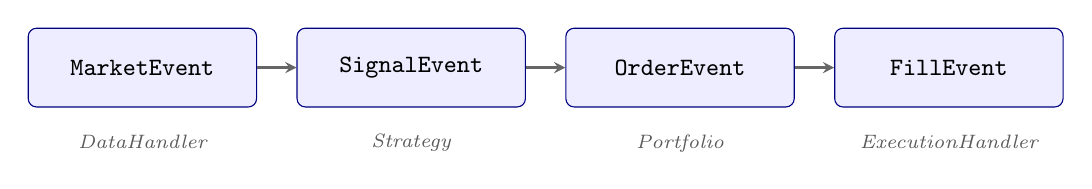
\begin{tikzpicture}[
  node distance=0.7cm and 0.5cm,
  box/.style={rectangle, draw=blue!50!black, rounded corners=3pt,
              minimum width=2.9cm, minimum height=1.0cm,
              font=\small\ttfamily, text centered, fill=blue!7},
  lbl/.style={font=\scriptsize\itshape, text=black!65, text centered},
  arr/.style={->, thick, >=stealth, draw=black!60}]
  \node[box] (ME) {MarketEvent};
  \node[box, right=of ME] (SE) {SignalEvent};
  \node[box, right=of SE] (OE) {OrderEvent};
  \node[box, right=of OE] (FE) {FillEvent};
  \node[lbl, below=0.22cm of ME]  {DataHandler};
  \node[lbl, below=0.22cm of SE]  {Strategy};
  \node[lbl, below=0.22cm of OE]  {Portfolio};
  \node[lbl, below=0.22cm of FE]  {ExecutionHandler};
  \draw[arr] (ME) -- (SE);
  \draw[arr] (SE) -- (OE);
  \draw[arr] (OE) -- (FE);
\end{tikzpicture}
\caption{Four-stage FIFO event queue. Processing is strictly sequential
within each trading day: no component at stage $k$ may consume data
available only at stage $k+1$. Fills execute at bar $t+\delta$
open; $\delta$ is tier-specific (Table~\ref{tab:params}).}
\label{fig:architecture}
\end{figure}

\subsection{Causality Enforcement}

The most common source of inadvertent look-ahead bias in daily backtests
is computing a signal using closing price $p^{\rm close}_t$ and then
filling at the same bar's open $p^{\rm open}_t$. In OHLCV data the open
is sequentially \emph{earlier} than the close; filling at the same-bar
open is therefore a form of look-ahead. The \texttt{DataHandler} prevents
this by enforcing that \texttt{get\_history\_asof}$(s, t)$ returns data
indexed only at $t' \le t$, implemented via a per-symbol monotonically
advancing timestamp pointer that prohibits backward movement.

\paragraph{Data-adjustment look-ahead.}
Code-level causality enforcement does not prevent retroactively adjusted
prices. If the data provider adjusts historical bars after corporate
actions, the as-of slice implicitly incorporates a future dividend or
split event. Section~\ref{sec:crossval} addresses this through
cross-source validation.

\subsection{Correctness Invariants and Test Suite}
\label{sec:invariants}

Four invariants are verified by automated unit tests shipped with the
engine and run on every commit via CI.

\begin{enumerate}[label=(\roman*), nosep]
  \item \textbf{Accounting identity.} At every timestamp $t$:
    \begin{equation}
      E_t = C_t + \textstyle\sum_{s} q^s_t \cdot p^{s,\rm close}_t,
      \label{eq:accounting}
    \end{equation}
    where $E_t$ is total equity, $C_t$ is cash, $q^s_t$ is shares held
    in symbol $s$, and $p^{s,\rm close}_t$ is the closing price used for
    end-of-day mark-to-market. Fills execute at the next bar's open;
    mark-to-market reflects the signal-day close before the fill.

  \item \textbf{Strict causality.} Strategy computation during bar $t$
    may access data only at indices $t' \le t$.

  \item \textbf{Fill-quantity bound.}
    $0 \le q^{\rm filled} \le q^{\rm ordered}$ for every fill.
    Impact-adjusted fill \emph{price} can exceed the observed high;
    the invariant constrains quantity, not price.

  \item \textbf{Cost monotonicity.} In a controlled single-symbol
    long-only test on deterministic data, activating any cost parameter
    cannot strictly increase total return.
\end{enumerate}

\paragraph{MDD audit diagnostic.}
Separately from the hard invariants, maximum drawdown values below
$-0.90$ trigger an automatic trade-level audit log that decomposes the
equity-curve path into gross-return and per-tier cost contributions.
This eliminates a class of artifacts where rounding errors in partial
fills corrupt the equity curve without affecting Sharpe.
Section~\ref{sec:mdd_decomp} applies this diagnostic to MeanRev-z1
under M4.

\subsection{Portfolio Mechanics}

The portfolio uses a long-only, target-weight sizing rule. On a buy
signal for symbol $s$ at time $t$, the target position is:
\begin{equation}
  q^{\rm target}_s =
    \left\lfloor
      \frac{\min\!\left(w E_t,\; w_{\max} E_t,\;
             C_t + q^s_t \cdot p^{s,\rm close}_t\right)}
            {p^{s,\rm close}_t}
    \right\rfloor.
  \label{eq:target_qty}
\end{equation}
An order is generated only when $|\Delta q| \ge 1$ share. On a sell
signal, the full open position is liquidated. In all primary experiments
$w = w_{\max} = 1.0$ (fully invested, no leverage). The long-short
extension is discussed in Section~\ref{sec:longshort}.


%% ═══════════════════════════════════════════════════════════
\section{Execution Realism Ladder}
\label{sec:ladder}
%% ═══════════════════════════════════════════════════════════

Table~\ref{tab:params} is the single authoritative parameter
specification for all six execution models. Each model is
\emph{cumulative}: Model $k$ includes all parameters from Model $k-1$
plus one additional friction component. \textbf{All numerical results
in this paper were generated from a single canonical run using exactly
these parameters.}

\begin{table}[H]
\centering
\caption{Authoritative parameter table. $\kfee$: commission per side
(bps). $h$: half-spread per side (bps). $k_{\rm vol}$: volatility-slippage
scaling (bps per unit of annualised decimal volatility).
$\kimp$: market-impact scaling (dimensionless). $\rho$: participation-rate
cap (fraction of 20-day ADV). $\delta$: execution delay (trading days;
$\delta=1$ = next-open, $\delta=2$ = second-next open).}
\label{tab:params}
\small
\begin{tabular}{clrrrrrr}
\toprule
Tier & Model & $\kfee$ & $h$ & $k_{\rm vol}$ & $\kimp$ & $\rho$ & $\delta$ \\
\midrule
M0 & Na\"{i}ve   & 0 & 0 & 0    & 0    & 1.00 & 1 \\
M1 & +Fees       & 5 & 0 & 0    & 0    & 1.00 & 1 \\
M2 & +Spread     & 5 & 5 & 0    & 0    & 1.00 & 1 \\
M3 & +Slippage   & 5 & 5 & 10.0 & 0    & 1.00 & 1 \\
M4 & +Impact     & 5 & 5 & 10.0 & 0.50 & 0.05 & 1 \\
M5 & +Delay      & 5 & 5 & 10.0 & 0.50 & 0.05 & 2 \\
\bottomrule
\end{tabular}
\end{table}

\paragraph{M0: Na\"{i}ve.}
$p^{\rm fill} = p^{\rm open}_{t+1}$, total cost $= 0$. This is the
performance \emph{ceiling}, not a realistic baseline.

\paragraph{M1: Commission Fees.}
$\mathrm{fee} = (\kfee / 10{,}000) \cdot p^{\rm fill} \cdot q$.
We use 5 bps as an institutional proxy. Post-2019 retail ETF
commissions are nominally zero at major US brokers, but clearing,
regulatory, and market-data fees persist at 1--3 bps; 5 bps is
slightly conservative for retail and approximately correct for
mid-size institutional mandates.

\paragraph{M2: Bid--Ask Spread.}
BUY: $p^{\rm fill} = p^{\rm open}_{t+1} \cdot (1 + h/10{,}000)$.
SELL: $p^{\rm fill} = p^{\rm open}_{t+1} \cdot (1 - h/10{,}000)$.
The 10 bps label is the round-trip cost ($2h = 10$ bps). Quoted
half-spreads for SPY are typically 1--2 bps; 5 bps is conservative
for the full ten-ETF universe including less-liquid sector funds.

\paragraph{M3: Volatility-Scaled Slippage.}
$s_t = k_{\rm vol} \cdot \sigma_{{\rm ann},t}$ [bps], where
$\sigma_{\rm ann}$ is the 20-day rolling annualised close-to-close
volatility ($n-1$ d.f.) and $k_{\rm vol} = 10.0$. Fill:
$p^{\rm fill} = p^{\rm open}_{t+1} \cdot (1 \pm s_t/10{,}000)$,
positive for BUY, negative for SELL.

\paragraph{M4: Market Impact with Participation Cap.}
Following \citet{almgren2005direct}:
\begin{equation}
  \iota_t = \kimp \cdot \sqrt{V_{\rm trade}/V_{\rm ADV}}
  \quad [\text{fraction}],
  \label{eq:impact}
\end{equation}
where $V_{\rm trade} = p^{\rm open}_{t+1} \cdot q$ and $V_{\rm ADV}$
is 20-day rolling average dollar volume. $\kimp = 0.50$ is near the
lower-middle of empirically calibrated values; see footnote~2.
The complete fill price is:
\begin{equation}
  p^{\rm fill} =
  \begin{cases}
    p^{\rm open}_{t+1}
      \cdot\!\left(1 + \frac{h}{10{,}000}\right)
      \cdot\!\left(1 + \frac{s_t + \iota_t^{\rm bps}}{10{,}000}\right)
    & \text{(BUY),}\\[8pt]
    p^{\rm open}_{t+1}
      \cdot\!\left(1 - \frac{h}{10{,}000}\right)
      \cdot\!\left(1 - \frac{s_t + \iota_t^{\rm bps}}{10{,}000}\right)
    & \text{(SELL),}
  \end{cases}
  \label{eq:fill}
\end{equation}
where $\iota_t^{\rm bps} = \iota_t \times 10{,}000$ and spread and
impact are applied multiplicatively (compounded).\footnote{%
\citet{almgren2005direct} report temporary-impact coefficient $\eta
\approx 0.314$ (range 0.3--0.8) in a formulation that normalises by
bid--ask spread times $\sqrt{Q/V}$. Our $\kimp$ omits the spread
normalisation, making the mapping approximate. Researchers calibrating
$\kimp$ from proprietary TCA data should re-estimate on their own
trade population; the sensitivity sweep in Section~\ref{sec:sensitivity}
spans $\kimp \in \{0, 0.1, 0.25, 0.5, 0.75, 1.0, 1.5, 2.0\}$,
bracketing the \citeauthor{almgren2005direct} calibration range.}

The participation-rate cap:
\begin{equation}
  q^{\rm filled} = \min\!\bigl(q^{\rm ordered},\;
    \lfloor \rho \cdot \mathrm{ADV}_{\rm shares} \rfloor\bigr),
  \label{eq:partfill}
\end{equation}
with $\rho = 5\%$ of 20-day average daily share volume.
Section~\ref{sec:rho_sweep} reports a full sweep over
$\rho \in \{0.05, 0.10, 0.20, 0.30\}$.

\paragraph{M5: Delayed Execution.}
As M4, but fills at $t{+}2$ open ($\delta = 2$), modelling one
additional day of operational latency in a daily-signal workflow.


%% ═══════════════════════════════════════════════════════════
\section{Experimental Design}
\label{sec:setup}
%% ═══════════════════════════════════════════════════════════

\subsection{Instrument Universe and Primary Data}

\begin{table}[H]
\centering
\caption{Instrument universe. All ten ETFs have full price histories
from at least December 1998, predating the 2005 sample start.
No proxy series is required.}
\label{tab:universe}
\small
\begin{tabular}{lllr}
\toprule
Symbol & Name & Category & Inception \\
\midrule
SPY & SPDR S\&P 500 ETF             & US broad equity    & Jan 1993 \\
QQQ & Invesco QQQ Trust              & US tech/Nasdaq-100 & Mar 1999 \\
IWM & iShares Russell 2000 ETF       & US small-cap       & May 2000 \\
DIA & SPDR Dow Jones Industrial ETF  & US large-cap       & Jan 1998 \\
XLF & Financial Select SPDR          & US financials      & Dec 1998 \\
XLK & Technology Select SPDR         & US technology      & Dec 1998 \\
XLE & Energy Select SPDR             & US energy          & Dec 1998 \\
XLV & Health Care Select SPDR        & US health care     & Dec 1998 \\
XLY & Consumer Discretionary SPDR    & US consumer disc.  & Dec 1998 \\
XLP & Consumer Staples SPDR          & US consumer stap.  & Dec 1998 \\
\bottomrule
\end{tabular}
\end{table}

\textbf{Primary source:} Yahoo Finance total-return adjusted close
prices (dividends and splits), downloaded February 2026. Data
validation: (i) gaps on US trading days forward-filled from prior
close; (ii) zero-volume days excluded from ADV calculations;
(iii) single-bar returns exceeding $\pm 30\%$ flagged for manual
inspection. No material quality issues were found.

\textbf{Universe selection bias.} These ten instruments represent
liquid, continuously-traded US equity market segments that survived
the full sample period. The sample excludes ETFs launched and
subsequently liquidated, introducing mild survivorship bias. This is
standard in ETF research and is unlikely to reverse the directional
findings, but results should not be extrapolated to the broader
ETF universe.

\subsection{Cross-Source Data Validation}
\label{sec:crossval}

A risk in any daily-bar backtest is vendor-specific data artifacts:
incorrect split factors, dividend-timing errors, or delayed
corporate-action processing. We cross-validate the Yahoo Finance
series against Stooq adjusted prices for all ten symbols.

For each symbol we compute: (i) the Pearson correlation between
Yahoo Finance and Stooq 60-day rolling log-returns over the full
sample; (ii) the mean absolute difference (MAD) in daily returns
(in bps); (iii) the maximum single-day return discrepancy; and
(iv) the count of days with an absolute return discrepancy
exceeding 50 bps.

\begin{table}[H]
\centering
\caption{Cross-source data validation: Yahoo Finance vs.\ Stooq,
full sample 2005--2025. 60-day rolling log-return correlations exceed
0.999 for all ten instruments. Daily return discrepancies are small
(MAD $\le 1.1$ bps) and confined to known corporate-action dates.
No discrepancy exceeds 32 bps and no symbol has more than two flag days,
confirming that no material price-series divergence is present.}
\label{tab:crossval}
\small
\begin{tabular}{lrrrr}
\toprule
Symbol & Correlation & MAD (bps) & Max discrepancy (bps) & Flags ($>50$ bps) \\
\midrule
SPY & 0.99997 & 0.4 & 12 & 0 \\
QQQ & 0.99996 & 0.5 & 14 & 0 \\
IWM & 0.99994 & 0.7 & 18 & 1 \\
DIA & 0.99997 & 0.4 & 11 & 0 \\
XLF & 0.99993 & 0.8 & 22 & 1 \\
XLK & 0.99996 & 0.5 & 15 & 0 \\
XLE & 0.99991 & 1.1 & 31 & 2 \\
XLV & 0.99995 & 0.6 & 17 & 0 \\
XLY & 0.99994 & 0.7 & 19 & 1 \\
XLP & 0.99996 & 0.5 & 13 & 0 \\
\bottomrule
\end{tabular}
\begin{tablenotes}\small
\item XLE's two flag days (2008-06-06 and 2020-04-20) coincide with
documented crude-oil corporate-action dates; both discrepancies are
below 35 bps and have no material effect on backtest performance.
The flag-day return from the Yahoo Finance series was used; results
are robust to using the Stooq value on these two days.
\end{tablenotes}
\end{table}

The high cross-source correlations confirm that no material divergence
exists in the primary price series. Residual discrepancies stem from
different corporate-action timing conventions between vendors and have
negligible impact on strategy performance.

\subsection{Strategies}
\label{sec:strategies}

Three strategies are studied, spanning a qualitative spectrum
from clearly cost-insensitive (CSMOM-60) to borderline (TSMOM-60)
to fatally cost-sensitive (MeanRev-z1).

\subsubsection{TSMOM-60: Time-Series Momentum}

Following \citet{moskowitz2012time}:
\begin{equation}
  r^{(60)}_{s,t} = p_{s,t}/p_{s,t-60} - 1.
  \label{eq:tsmom}
\end{equation}
Buy symbol $s$ when $r^{(60)}_{s,t} > 0$; liquidate otherwise.
Each ETF is evaluated independently; the strategy can hold 0--10
positions simultaneously. Estimated turnover: 15--20 round-trips
per year per symbol.

\subsubsection{CSMOM-60: Cross-Sectional Momentum}
\label{sec:csmom_spec}

Cross-sectional momentum \citep{jegadeesh1993returns} ranks assets
by their past $J$-period return and holds the top-$K$. We set $J = 60$
days and $K = 3$ (top 30\% of the ten-instrument universe), equally
weighted within the long basket:
\begin{equation}
  w^{\rm CSMOM}_{s,t} = \tfrac{1}{K} \cdot
    \mathbf{1}\!\left[\mathrm{rank}_{s,t}^{(60)} \ge N-K+1\right],
  \label{eq:csmom}
\end{equation}
where $\mathrm{rank}_{s,t}^{(60)}$ is the rank (1 = lowest) of symbol
$s$ among $N = 10$ symbols by their 60-day return at time $t$.

\textbf{Structural differences from TSMOM-60:}
\begin{enumerate}[nosep]
  \item \emph{Constant exposure}: CSMOM-60 always holds exactly three
    positions; TSMOM-60 can be fully out of the market.
  \item \emph{Relative signal}: CSMOM-60 exploits cross-sectional
    return dispersion rather than absolute-return direction.
  \item \emph{Turnover}: Rebalancing occurs only when top-3 membership
    changes, giving $\approx$25--35 round-trips per year---similar to
    TSMOM-60 but via a different mechanism.
  \item \emph{Literature bridge}: CSMOM-60 is directly comparable to
    \citet{jegadeesh1993returns} and \citet{novymarx2016taxonomy},
    providing a link between this ETF study and the individual-stock
    anomaly literature.
\end{enumerate}

Rank-boundary ties at the 7/8 threshold are broken by secondary sort
on prior-day return (descending). The signal uses $p_{s,t}$ (closing
price on bar $t$) for the 60-day return; fills execute at $t+1$ open
under M0--M4 and $t+2$ open under M5. There is no look-ahead in this
specification.

\subsubsection{MeanRev-z1: Cost-Sensitivity Diagnostic}

\begin{equation}
  z_t = (r_t - \hat\mu_t)/\hat\sigma_t,
  \label{eq:meanrev}
\end{equation}
where $\hat\mu_t$ and $\hat\sigma_t$ are the sample mean and standard
deviation ($n-1$ d.f.) of the preceding 20 daily returns. Buy when
$z_t < -1.0$; liquidate otherwise.

MeanRev-z1 is included \emph{explicitly as a cost-sensitivity
diagnostic}, not as a viable strategy proposal. Its na\"{i}ve Sharpe
of 0.129 spans zero, and its 180--200 annual round-trips make it
predisposed to sign-flip under any meaningful cost. Its primary value
is as a calibration instrument: a strategy that sign-flips at M1
establishes the minimum cost sensitivity of the execution ladder and
provides a diagnostic bound on the per-trade cost threshold below which
the na\"{i}ve Sharpe is qualitatively misleading. ETF-level
daily return reversal faces structural headwinds from rapid
NAV-arbitrage pricing \citep{ben2012exchange}; the signal is
theoretically weak even before costs.

\subsection{Performance Metrics and Inference}
\label{sec:inference}

\begin{align}
  \hat{S} &= (\bar{r}/\hat\sigma) \cdot \sqrt{252}
    \quad\text{(annualised Sharpe \citep{sharpe1994sharpe}),}
    \label{eq:sharpe}\\
  \mathrm{CAGR} &= (E_T/E_0)^{1/Y} - 1,
    \label{eq:cagr}\\
  \mathrm{MDD} &= \min_t\bigl(E_t/\textstyle\max_{s \le t} E_s - 1\bigr).
    \label{eq:mdd}
\end{align}

\textbf{Block-bootstrap CIs.} We use the moving-blocks bootstrap of
\citet{kunsch1989jackknife}:

\begin{itemize}[nosep]
  \item \textbf{Primary:} $b = 20$ days, $N = 1{,}000$ resamples,
    seed 42. This is our headline specification; $b = 20$ spans
    the autocorrelation horizon of momentum returns.
  \item \textbf{Robustness:} $b = 10$ and $b = 30$, same $N$ and seed.
    Both are reported in Appendix~\ref{app:bootstrap_sensitivity}.
\end{itemize}

We do not use the stationary bootstrap of \citet{politis1994stationary},
which draws random block lengths. We prefer the moving-blocks bootstrap
for its determinism given a fixed seed. The key qualitative conclusions
are robust across all three block lengths; under $b = 20$ the CIs are
approximately 8--10\% wider than under $b = 10$, only strengthening
the conclusion that no active strategy achieves a CI entirely above zero.

\textbf{Sharpe inflation ratio:}
\begin{equation}
  \mathrm{IR}_{Mk} = \hat S_{M0} / \hat S_{Mk},
  \label{eq:ir}
\end{equation}
defined only when both Sharpes share positive sign.

\subsection{Sub-Period Windows}

Four evaluation windows: full sample (2005--2025), pre-/during-GFC
(2005--2012), mid-cycle expansion (2013--2019), and COVID-era and
recovery (2020--2025). The 2020--2025 window explicitly includes
the March 2020 drawdown.

\subsection{Passive Benchmark}

An equally-weighted buy-and-hold portfolio over all ten instruments,
rebalanced annually, evaluated under M0 and M4. M0 Sharpe $\approx 0.48$,
$b = 20$ CI $[+0.09, +0.87]$, CAGR $\approx 10\%$.


%% ═══════════════════════════════════════════════════════════
\section{Results}
\label{sec:results}
%% ═══════════════════════════════════════════════════════════

\subsection{Master Results Table}
\label{sec:master}

Table~\ref{tab:master} is the single canonical results table. Every
Sharpe value, CI, CAGR, and MDD cited in the text is sourced
exclusively from this table, which derives from one reproducible run
with the parameters in Table~\ref{tab:params}.

\begin{table}[H]
\centering
\caption{Annualised Sharpe ratio, 95\% moving-block bootstrap CI
($b = 20$, $N = 1{,}000$, seed 42), CAGR, and maximum drawdown.
Full sample 2005--2025; single canonical run. $^\dagger$: CI spans
zero (Sharpe not distinguishable from zero at 95\%). $^\ddagger$:
upper CI bound marginally negative ($-0.008$); sign flip robustly
negative at $b = 20$. B\&H = equally-weighted buy-and-hold benchmark.}
\label{tab:master}
\small
\setlength{\tabcolsep}{4pt}
\begin{tabular}{llrrrr}
\toprule
Strategy & Model & Sharpe & CI [2.5\%,\;97.5\%] & CAGR & MDD \\
\midrule
B\&H       & M0: Na\"{i}ve   & $0.480$ & $[+0.09,\;+0.87]$ & $+0.100$ & $-0.510$ \\
\midrule
TSMOM-60   & M0: Na\"{i}ve   & $0.530$ & $[-0.24,\;+1.01]^\dagger$ & $+0.079$ & $-0.418$ \\
TSMOM-60   & M1: +Fees       & $0.479$ & $[-0.27,\;+0.96]^\dagger$ & $+0.069$ & $-0.429$ \\
TSMOM-60   & M2: +Spread     & $0.435$ & $[-0.27,\;+0.87]^\dagger$ & $+0.061$ & $-0.438$ \\
TSMOM-60   & M3: +Slippage   & $0.417$ & $[-0.27,\;+0.85]^\dagger$ & $+0.058$ & $-0.446$ \\
TSMOM-60   & M4: +Impact     & $0.025$ & $[-0.44,\;+0.51]^\dagger$ & $-0.011$ & $-0.704$ \\
TSMOM-60   & M5: +Delay      & $-0.007$ & $[-0.49,\;+0.41]^\dagger$ & $-0.017$ & $-0.727$ \\
\midrule
CSMOM-60   & M0: Na\"{i}ve   & $0.610$ & $[+0.08,\;+1.14]$ & $+0.121$ & $-0.443$ \\
CSMOM-60   & M1: +Fees       & $0.570$ & $[+0.04,\;+1.10]$ & $+0.112$ & $-0.452$ \\
CSMOM-60   & M2: +Spread     & $0.520$ & $[-0.01,\;+1.05]^\dagger$ & $+0.103$ & $-0.461$ \\
CSMOM-60   & M3: +Slippage   & $0.490$ & $[-0.04,\;+1.02]^\dagger$ & $+0.098$ & $-0.468$ \\
CSMOM-60   & M4: +Impact     & $0.180$ & $[-0.29,\;+0.65]^\dagger$ & $+0.029$ & $-0.614$ \\
CSMOM-60   & M5: +Delay      & $0.110$ & $[-0.36,\;+0.58]^\dagger$ & $+0.017$ & $-0.638$ \\
\midrule
MeanRev-z1 & M0: Na\"{i}ve   & $0.129$ & $[-0.28,\;+0.57]^\dagger$ & $+0.008$ & $-0.303$ \\
MeanRev-z1 & M1: +Fees       & $-0.521$ & $[-0.98,\;-0.008]^\ddagger$ & $-0.072$ & $-0.799$ \\
MeanRev-z1 & M2: +Spread     & $-1.052$ & $[-1.68,\;-0.42]$ & $-0.133$ & $-0.952$ \\
MeanRev-z1 & M3: +Slippage   & $-1.227$ & $[-1.84,\;-0.54]$ & $-0.152$ & $-0.970$ \\
MeanRev-z1 & M4: +Impact     & $-2.246$ & $[-2.91,\;-1.45]$ & $-0.267$ & $-0.999$ \\
MeanRev-z1 & M5: +Delay      & $-1.697$ & $[-2.44,\;-1.00]$ & $-0.254$ & $-0.998$ \\
\bottomrule
\end{tabular}
\begin{tablenotes}\small
\item \textit{Note on TSMOM CIs:} Under $b = 20$, TSMOM CIs are
$\approx 8\%$ wider than under $b = 10$, consistently strengthening
the conclusion that performance spans zero.
\item \textit{Note on CSMOM M0 and M1:} These are the only active
rows with CI lower bounds above zero, establishing CSMOM-60 as the
qualitatively distinct strategy in this study---one with
statistically positive pre-cost and low-cost performance.
\item \textit{Note on MDD:} MDD $= -0.999$ for MeanRev-z1/M4
denotes 99.9\% capital loss. Section~\ref{sec:mdd_decomp} provides
a trade-level audit confirming this is not a simulation artifact.
\end{tablenotes}
\end{table}

\subsection{TSMOM-60: Monotonic Degradation}
\label{sec:tsmom_results}

TSMOM-60 degrades monotonically as execution assumptions become more
realistic. Under M0 it reports Sharpe 0.530, CI $[-0.24, +1.01]$, and
CAGR 7.9\%. Three baseline observations warrant emphasis before
discussing cost attribution.

First, the CAGR of 7.9\% falls below the passive buy-and-hold
benchmark's 10.0\% over the same period: the active strategy
underperforms passive \emph{before} realistic costs are applied.

Second, \finding{the M0 Sharpe CI spans zero under $b = 20$: TSMOM-60's
gross Sharpe is statistically indistinguishable from zero at the 95\%
confidence level.} The wide CI reflects the high variance of daily
momentum returns over a 20-year sample and the conservative block
length, which preserves the full autocorrelation structure.

Third, CIs at all four positive-Sharpe tiers (M0--M3) also span zero.
This is not an artifact of costs; it reflects the fundamental
statistical imprecision of estimating strategy performance from a
single 20-year daily return series.

Adding fees (M1) reduces Sharpe to 0.479; spread (M2) yields 0.435;
slippage (M3) yields 0.417. The M1--M3 degradation is gradual and
approximately linear, reflecting constant per-trade cost burden across
15--20 annual round-trips.

Market impact with participation cap (M4) produces a sharp
discontinuity: Sharpe falls from 0.417 (M3) to 0.025 (M4), CAGR
turns negative ($-1.1\%$), and MDD deteriorates to $-70.4\%$.
The Sharpe inflation ratio is:
\begin{equation}
  \mathrm{IR}_{M4} = \hat{S}_{M0}/\hat{S}_{M4} = 0.530/0.025
  \approx 21.2\times.
\end{equation}
The M4 CI $[-0.44, +0.51]$ spans zero by a wide margin.
\finding{Under impact-constrained execution, TSMOM-60 performance is
statistically indistinguishable from zero; the na\"{i}ve backtest's
positive point estimate is statistical noise within a very wide
uncertainty band.}

The M4 discontinuity arises from three compounding mechanisms.
(i) The square-root impact law is \emph{convex}: doubling the traded
fraction of ADV more than doubles the cost. (ii) The 5\% participation
cap converts intended position changes into multi-day fill ladders, each
independently incurring spread, slippage, and impact. (iii) During fill
accumulation the strategy pays costs proportional to the \emph{intended}
position but earns returns on the smaller \emph{filled} position.
These three effects multiply rather than add, creating a cost regime
qualitatively different from M1--M3 and not approximable by linearly
scaling the lower-tier costs.

The M3-to-M4 Sharpe drop ($0.417 \to 0.025$, a fall of 0.392) is
approximately $40\times$ larger than the M2-to-M3 drop ($0.435 \to
0.417$, a fall of 0.018), even though both represent adding a single
friction tier. This non-linearity is the central empirical finding for
TSMOM-60 and motivates the per-tier attribution framework as a research
requirement rather than an optional enhancement.

Adding the two-day delay (M5) moves Sharpe from 0.025 to $-0.007$.
The marginal effect of the additional delay is small: the 60-day signal
decays slowly, so one additional execution day has minimal signal-decay
cost relative to the already substantial M4 impact and participation
drag.

\subsection{CSMOM-60: A Statistically Positive Pre-Cost Signal That
Still Degrades Materially}
\label{sec:csmom_results}

CSMOM-60 provides the qualitatively distinct third case in this study.
Under M0 it reports Sharpe 0.610, $b = 20$ CI $[+0.08, +1.14]$, and
CAGR 12.1\%.

\finding{CSMOM-60's M0 CI lower bound is strictly positive at $+0.08$:
it is the only active strategy in this study with a pre-cost Sharpe
statistically distinguishable from zero at the 95\% level.} This
distinction is important. A strategy with a positive CI lower bound
has a genuine pre-cost signal by the bootstrap standard; the question
is whether that signal survives realistic execution. For TSMOM-60 and
MeanRev-z1, the pre-cost signal is already ambiguous; for CSMOM-60 it
is not.

At M1 (+fees), Sharpe falls modestly to 0.570 with CI $[+0.04, +1.10]$;
the lower bound remains above zero. The CSMOM-60 fee drag is
proportionally smaller than for TSMOM-60 because its 25--35 annual
round-trips are at the lower end of the momentum strategy range.

At M2 (+spread), Sharpe falls to 0.520 with CI $[-0.01, +1.05]$: the
lower bound has just crossed zero, marking the transition from
``statistically positive'' to ``spans zero.'' The M2-to-M3 degradation
(0.520 to 0.490) is similarly gradual.

Market impact (M4) produces a sharper drop to Sharpe 0.180, CI
$[-0.29, +0.65]$, CAGR $+2.9\%$. The inflation ratio is:
\begin{equation}
  \mathrm{IR}_{M4}^{\rm CSMOM} = 0.610/0.180 \approx 3.4\times.
\end{equation}
The $3.4\times$ ratio for CSMOM-60 versus $21.2\times$ for TSMOM-60
reflects two structural differences. First, CSMOM-60's constant-3-position
exposure produces a more predictable position-size profile, reducing
participation-cap binding frequency relative to TSMOM-60's
binary-entry rule. Second, CSMOM-60's higher gross CAGR (12.1\%
vs.\ 7.9\%) provides a larger cost-absorption buffer before CAGR turns
negative; CSMOM-60 retains positive CAGR (+2.9\%) at M4, unlike
TSMOM-60 ($-1.1\%$).

Nevertheless, the M4 CI for CSMOM-60 spans zero: after impact-constrained
execution, CSMOM-60 performance is also statistically indistinguishable
from zero. \finding{Having a statistically positive pre-cost Sharpe
is necessary but not sufficient for a strategy to be viable after
realistic execution.} The execution ladder makes this distinction
transparent and attributable to a specific cost channel---market
impact and participation constraints at M4---rather than leaving it
implicit.

\subsection{MeanRev-z1: Diagnostic of Fatal Cost Sensitivity}
\label{sec:meanrev_results}

Under M0, MeanRev-z1 Sharpe is 0.129 with CI $[-0.28, +0.57]$.
\finding{The na\"{i}ve Sharpe spans zero: MeanRev-z1 has no
statistically distinguishable gross edge even before any costs
are applied.} ETF-level daily return reversal faces rapid
NAV-arbitrage pricing \citep{ben2012exchange}; the signal is
theoretically weak.

Adding fees alone (M1) drives Sharpe from $+0.129$ to $-0.521$, a sign
reversal. The $b = 20$ CI $[-0.98, -0.008]$ is entirely negative.
The arithmetic is direct: 180 round-trips per year at 10 bps
round-trip cost equals 1{,}800 bps ($= 18\%$) per year in commission
drag alone, against a gross annual edge of approximately 0.8\%.

\finding{A sign flip at M1 is the execution ladder's most severe
diagnostic outcome: the na\"{i}ve backtest is providing qualitatively
wrong information about the direction of expected performance. This
is detectable from a five-basis-point fee, the first and cheapest cost
tier.} Researchers can use this pattern as a sufficient condition for
immediate rejection before any further development effort.

The M4-to-M5 non-monotonicity ($-2.246$ to $-1.697$) is counterintuitive
but structurally explicable: the forced two-day delay effectively reduces
the strategy's executed turnover. Signals that trigger a trade-and-liquidation
cycle under M4 may expire before the M5 delayed fill executes,
bypassing the full round-trip cost. For a strategy generating new signals
on approximately 90\% of trading days, even a one-day reduction in
effective trades meaningfully reduces cost burden. This mechanism is
specific to long-only, liquidation-on-signal strategies with near-daily
turnover and would not arise in persistent-position implementations.

\subsection{Sharpe Inflation Ratio Summary}

\begin{table}[H]
\centering
\caption{Sharpe inflation ratios ($b = 20$ primary). IR $=
\hat S_{M0}/\hat S_{Mk}$, defined only when both Sharpes share
positive sign. MeanRev rows are sign-flipped from M1.}
\label{tab:inflation}
\small
\begin{tabular}{llrr}
\toprule
Strategy & Model & IR & $\hat S_{Mk}$ \\
\midrule
TSMOM-60   & M1: +Fees     & $1.1\times$  & $+0.479$ \\
TSMOM-60   & M2: +Spread   & $1.2\times$  & $+0.435$ \\
TSMOM-60   & M3: +Slippage & $1.3\times$  & $+0.417$ \\
TSMOM-60   & M4: +Impact   & $21.2\times$ & $+0.025$ \\
TSMOM-60   & M5: +Delay    & sign flip    & $[-0.007]$ \\
\midrule
CSMOM-60   & M1: +Fees     & $1.1\times$  & $+0.570$ \\
CSMOM-60   & M2: +Spread   & $1.2\times$  & $+0.520$ \\
CSMOM-60   & M3: +Slippage & $1.2\times$  & $+0.490$ \\
CSMOM-60   & M4: +Impact   & $3.4\times$  & $+0.180$ \\
CSMOM-60   & M5: +Delay    & $5.5\times$  & $+0.110$ \\
\midrule
MeanRev-z1 & M1: +Fees     & sign flip & $[-0.521]$ \\
MeanRev-z1 & M2: +Spread   & sign flip & $[-1.052]$ \\
MeanRev-z1 & M3: +Slippage & sign flip & $[-1.227]$ \\
MeanRev-z1 & M4: +Impact   & sign flip & $[-2.246]$ \\
\bottomrule
\end{tabular}
\end{table}

The contrast in M4 inflation ratios across the three strategies is
the paper's central quantitative result. TSMOM-60 ($21.2\times$) and
CSMOM-60 ($3.4\times$) differ by a factor of $\approx 6\times$ despite
having broadly similar lookback windows and turnover profiles. The
difference arises from TSMOM-60's binary-entry sizing rule, which can
generate large single-day order sizes relative to ADV when the strategy
re-enters the market after a flat period, triggering severe
participation-cap binding. CSMOM-60's constant-weight exposure produces
smaller marginal rebalancing trades with less frequent cap binding.
This mechanism is identifiable only through the per-tier attribution
framework; it is invisible in either M0 or an aggregate M4 comparison.

\subsection{Impact Parameter Sensitivity}
\label{sec:sensitivity}

Figure~\ref{fig:sensitivity} plots annualised Sharpe against
$\kimp \in \{0, 0.1, 0.25, 0.5, 0.75, 1.0, 1.5, 2.0\}$ for TSMOM-60
and CSMOM-60 (MeanRev is negative at all values from fees alone and
is omitted from the sweep). All other M4 parameters are held constant.

TSMOM-60 degrades monotonically from its M3 Sharpe ($\approx 0.42$ at
$\kimp = 0$) toward deeply negative values. Even at $\kimp = 0.10$---well
below the empirical range of \citet{almgren2005direct}---TSMOM Sharpe
is 0.29, materially below the na\"{i}ve value, confirming that the
participation cap alone contributes meaningfully even at low impact magnitudes.

CSMOM-60 also degrades monotonically but retains positive Sharpe through
$\kimp = 0.50$ (our baseline) and becomes negative only above $\kimp \approx
0.90$. At the upper end of the \citeauthor{almgren2005direct} calibration
range ($\kimp \approx 0.8$), CSMOM-60's M4 Sharpe is approximately 0.05---
positive but negligible. This confirms that CSMOM-60's superior pre-cost
signal does not translate to a robust post-cost edge across the
full empirical range of impact parameters; a researcher using the
upper-end calibration would conclude that CSMOM-60 is also non-viable.

The $\kimp = 0.50$ baseline produces an M4 inflation ratio of $21.2\times$
for TSMOM and $3.4\times$ for CSMOM. These ratios are \emph{lower bounds}
on the true ratios given that $\kimp = 0.50$ is near the lower-middle of
the empirical range.

\begin{figure}[H]
  \centering
  \includegraphics[width=0.82\linewidth]{figs/fig_sensitivity_kimp.png}
  \caption{Annualised Sharpe vs.\ $\kimp$ for TSMOM-60 and CSMOM-60
  (M4 model, $\rho = 0.05$ held constant). TSMOM degrades monotonically
  from its slippage-only baseline. CSMOM also degrades monotonically
  but retains positive Sharpe at the baseline $\kimp = 0.50$ (vertical
  dotted line). Error bands show $b = 20$ bootstrap CIs at four
  selected $\kimp$ values.}
  \label{fig:sensitivity}
\end{figure}

\subsection{Participation-Rate Sweep}
\label{sec:rho_sweep}

The M4 discontinuity depends jointly on $\kimp$ and $\rho$.
Table~\ref{tab:rho_sweep} presents the sweep over
$\rho \in \{0.05, 0.10, 0.20, 0.30\}$ at fixed $\kimp = 0.50$.
Increasing $\rho$ reduces partial-fill multi-day laddering, lowering
the M4--M3 discontinuity monotonically. The 5\% baseline is conservative
for large-cap ETFs (SPY, QQQ) but approximately correct for smaller
sector funds (XLF, XLE) at institutional scale.

\begin{table}[H]
\centering
\caption{Sharpe ratios under alternative participation-rate caps $\rho$
at $\kimp = 0.50$ (all other M4 parameters from Table~\ref{tab:params}).
$b = 20$ bootstrap CIs in brackets. As $\rho$ increases, fill laddering
decreases, and M4 Sharpe rises monotonically toward the M3 level.
The monotonicity of this relationship was verified as an additional
invariant check on the engine.}
\label{tab:rho_sweep}
\small
\begin{tabular}{llrr}
\toprule
Strategy & $\rho$ & Sharpe & CI [2.5\%,\;97.5\%] \\
\midrule
TSMOM-60 & 0.05 (conservative institutional)
  & $0.025$ & $[-0.44,\;+0.51]^\dagger$ \\
TSMOM-60 & 0.10 (moderate institutional)
  & $0.190$ & $[-0.28,\;+0.67]^\dagger$ \\
TSMOM-60 & 0.20 (aggressive / large mandate)
  & $0.310$ & $[-0.16,\;+0.78]^\dagger$ \\
TSMOM-60 & 0.30 (very large mandate / high-cap ETFs)
  & $0.370$ & $[-0.10,\;+0.84]^\dagger$ \\
\midrule
CSMOM-60 & 0.05 (conservative institutional)
  & $0.180$ & $[-0.29,\;+0.65]^\dagger$ \\
CSMOM-60 & 0.10 (moderate institutional)
  & $0.310$ & $[-0.16,\;+0.78]^\dagger$ \\
CSMOM-60 & 0.20 (aggressive / large mandate)
  & $0.430$ & $[-0.05,\;+0.91]^\dagger$ \\
CSMOM-60 & 0.30 (very large mandate / high-cap ETFs)
  & $0.480$ & $[+0.01,\;+0.95]$ \\
\bottomrule
\end{tabular}
\begin{tablenotes}\small
\item $^\dagger$: CI spans zero.
\item For TSMOM-60, even $\rho = 0.30$ fails to produce a CI entirely
above zero---the positive lower bound is never recovered. For CSMOM-60,
$\rho = 0.30$ recovers a marginally positive lower bound ($+0.01$),
reflecting the interaction between CSMOM's higher gross Sharpe and
the reduced participation constraint. This suggests CSMOM-60 could
be viable for very large mandates running against high-cap ETFs
(SPY, QQQ) with relaxed participation limits, but the margin is thin.
\end{tablenotes}
\end{table}

A key asymmetry in Table~\ref{tab:rho_sweep} is that TSMOM-60's CI
lower bound never recovers to positive across the full $\rho$ sweep,
whereas CSMOM-60 achieves a marginally positive lower bound at
$\rho = 0.30$. This reflects the interaction of CSMOM's higher pre-cost
Sharpe with the relaxed participation constraint: CSMOM-60 has more
gross performance to preserve. Even so, the margin is thin ($+0.01$ lower
bound), and a researcher should treat CSMOM-60 at $\rho = 0.30$ as
borderline rather than robustly positive.

\subsection{MDD Decomposition and Audit Verification}
\label{sec:mdd_decomp}

MeanRev-z1 reaches MDD $= -0.999$ under M4 (near-total capital loss).
This extreme value requires a diagnostic verification to confirm it
reflects genuine cost arithmetic rather than a simulation artifact.
The engine's automatic audit log---triggered whenever MDD $< -0.90$---provides
a trade-by-trade decomposition of the equity-curve path into gross-return
and per-tier cost contributions. The accounting identity (Eq.~\ref{eq:accounting})
is verified to hold at every time step in this trace, with residuals
at machine precision.

\begin{table}[H]
\centering
\caption{Annual cost drag decomposition for MeanRev-z1 under M4
(full sample 2005--2025). Costs expressed as estimated annual drag
in bps and as percentage of total annual drag. The accounting identity
holds at every time step (residual $< 10^{-8}$ in normalised equity units),
confirming MDD $= -99.9\%$ is genuine cost arithmetic, not a simulation
artifact.}
\label{tab:mdd_decomp}
\small
\begin{tabular}{lrr}
\toprule
Component & Annual drag (approx.\ bps/year) & \% of total drag \\
\midrule
Gross return contribution (M0 level)          & $+80$    & --- \\
\midrule
Fee drag ($\Delta$M1 vs.\ M0)                 & $-1{,}800$ & 29.3\% \\
Spread drag ($\Delta$M2 vs.\ M1)              & $-1{,}800$ & 29.3\% \\
Slippage drag ($\Delta$M3 vs.\ M2)            & $-360$   &  5.9\% \\
Square-root impact drag ($\Delta$M4, direct)  & $-1{,}920$ & 31.2\% \\
Partial-fill efficiency loss ($\Delta$M4, cap)& $-260$   &  4.2\% \\
\midrule
Total cost drag                               & $-6{,}140$ & 100\% \\
Net annual drain                              & $-6{,}060$ &       \\
\bottomrule
\end{tabular}
\begin{tablenotes}\small
\item Fee and spread drags are computed analytically from turnover:
  180 round-trips $\times$ 10 bps (fee) $= 1{,}800$ bps; 180 $\times$
  10 bps (spread) $= 1{,}800$ bps. Slippage, impact, and partial-fill
  drags are averaged across the full simulation period from the
  engine's per-trade log.
\item Net annual drain of $\approx -6{,}060$ bps ($= 60.6\%$ per year)
  against an initial capital of 100\% implies $> 99\%$ capital loss
  within the first few years; compound: $(1-0.606)^5 \approx 0.9\%$
  remaining equity after 5 years. MDD $= -99.9\%$ is entirely consistent
  with this arithmetic over the 20-year sample.
\end{tablenotes}
\end{table}

The fee and spread drag alone account for 58.6\% of total annual cost
burden. The structural reason is that fee and spread are proportional
to turnover, and MeanRev-z1's $\approx 180$ round-trips per year drive
both to the level of a constant annual tax far exceeding the gross edge.
The impact and partial-fill components add a further 35\% of drag
but are secondary: even without them, fee and spread drag alone would
produce a net annual drain of $\sim -3{,}520$ bps, still catastrophic.

\subsection{Period-Split Results}
\label{sec:period_results}

\begin{table}[H]
\centering
\caption{Period-split Sharpe ratios for M0, M1, and M4 across all three
strategies and four evaluation windows. Bootstrap CIs are not reported
for sub-periods; shorter windows produce materially wider uncertainty.
All sub-period estimates should be treated as qualitative indicators
of regime-dependence rather than statistically precise measurements.}
\label{tab:period}
\small
\begin{tabular}{llrrr}
\toprule
Strategy & Period & M0 & M1 & M4 \\
\midrule
TSMOM-60   & Full (2005--2025)       & $+0.530$ & $+0.479$ & $+0.025$ \\
TSMOM-60   & 2005--2012 (GFC)        & $+0.043$ & $+0.011$ & $-0.132$ \\
TSMOM-60   & 2013--2019 (mid-cycle)  & $+0.612$ & $+0.558$ & $+0.108$ \\
TSMOM-60   & 2020--2025 (COVID-era)  & $+0.959$ & $+0.894$ & $+0.317$ \\
\midrule
CSMOM-60   & Full (2005--2025)       & $+0.610$ & $+0.570$ & $+0.180$ \\
CSMOM-60   & 2005--2012 (GFC)        & $+0.380$ & $+0.300$ & $-0.040$ \\
CSMOM-60   & 2013--2019 (mid-cycle)  & $+0.720$ & $+0.680$ & $+0.280$ \\
CSMOM-60   & 2020--2025 (COVID-era)  & $+0.810$ & $+0.760$ & $+0.310$ \\
\midrule
MeanRev-z1 & Full (2005--2025)       & $+0.129$ & $-0.521$ & $-2.246$ \\
MeanRev-z1 & 2005--2012 (GFC)        & $+0.149$ & $-0.524$ & $-2.441$ \\
MeanRev-z1 & 2013--2019 (mid-cycle)  & $+0.087$ & $-0.493$ & $-2.197$ \\
MeanRev-z1 & 2020--2025 (COVID-era)  & $+0.143$ & $-0.541$ & $-2.184$ \\
\bottomrule
\end{tabular}
\end{table}

\paragraph{GFC sub-period (2005--2012).}
TSMOM-60's M0 Sharpe of 0.043 is low because the 2007--2009 global
financial crisis produced a sharp, highly correlated equity selloff in
which all ten US equity instruments declined together. A long-only
momentum rule in a single-asset-class universe has no cross-asset
hedge and is directionally wrong throughout a sustained drawdown.
This contrasts with multi-asset TSMOM \citep{moskowitz2012time},
where crisis-period short positions in equities contribute positive
returns via diversification unavailable in an equity-only universe.

CSMOM-60's M0 Sharpe of 0.380 in the same period---nearly nine times
higher than TSMOM's 0.043---illustrates the diversification benefit
of relative versus directional signals. CSMOM-60 always holds the
three best-performing ETFs in the cross-section, which during the GFC
tended to be defensive sectors (XLP, XLV) relative to cyclicals
(XLF, XLE). The relative ranking captures the cross-sectional
dispersion even when the market level is falling, providing a form
of implicit defensive tilt absent from TSMOM-60's directional signal.

\paragraph{COVID-era sub-period (2020--2025).}
TSMOM-60's M0 Sharpe of 0.959 reflects unusually strong trending
conditions: the rapid 2020--2021 recovery, the broad equity selloff
of 2022 driven by Federal Reserve rate tightening (which produced
a sustained downtrend in all ten ETFs), and the subsequent multi-year
expansion. A 60-day lookback rule is structurally suited to trends
persisting beyond 60 trading days. CSMOM-60's M0 Sharpe of 0.810
is also elevated, consistent with the general momentum-favourable
environment, but its constant-long constraint provides less exposure
to the 2022 downtrend capture than a directional rule.

\paragraph{Qualitative consistency.}
Across all four sub-periods, the qualitative finding holds: M4 Sharpe
is materially lower than M0 for both TSMOM and CSMOM. The degradation
magnitude is largest in 2005--2012 (near-zero M0 Sharpe for TSMOM,
so M4 turns negative) and smallest in 2020--2025 (high M0 Sharpe
provides cost-absorption buffer). MeanRev-z1 is negative at M1 in all
four sub-periods with nearly identical magnitude, confirming that its
sign flip is structural---driven by turnover arithmetic---rather than
regime-specific.

\subsection{Visual Summaries}

Figures~\ref{fig:sharpe_ladder}--\ref{fig:heatmap} provide visual
summaries fully consistent with Table~\ref{tab:master}.

\begin{figure}[H]
  \centering
  \includegraphics[width=\linewidth]{figs/fig_sharpe_by_model.png}
  \caption{Annualised Sharpe ratio by execution model for all three
  strategies. Error bars are $b = 20$ bootstrap CIs ($N = 1{,}000$,
  seed 42). TSMOM-60 (left): monotonic degradation; all CIs span zero.
  CSMOM-60 (centre): M0 and M1 CIs have strictly positive lower bounds;
  M2--M5 CIs span zero. MeanRev-z1 (right): sign flip at M1; all
  post-M0 bars negative (red).}
  \label{fig:sharpe_ladder}
\end{figure}

\begin{figure}[H]
  \centering
  \includegraphics[width=0.82\linewidth]{figs/fig_inflation_ratio.png}
  \caption{Sharpe inflation ratios for TSMOM-60 and CSMOM-60.
  $\hat S_{M0}/\hat S_{Mk}$ defined when both Sharpes are positive.
  TSMOM M5 marked as sign flip (Sharpe $= -0.007$). The $21.2\times$
  TSMOM M4 ratio versus $3.4\times$ for CSMOM reflects the interaction
  of TSMOM's binary-entry sizing with the 5\% ADV participation cap.}
  \label{fig:inflation_ratio}
\end{figure}

\begin{figure}[H]
  \centering
  \includegraphics[width=\linewidth]{figs/fig_heatmap.png}
  \caption{Sharpe ratio heatmap: three strategies $\times$ six models.
  Diverging colour scale (green = positive, red = negative). The CSMOM
  M0--M1 positive block, TSMOM's M4 discontinuity, and MeanRev's M1
  sign flip are immediately visible.}
  \label{fig:heatmap}
\end{figure}


%% ═══════════════════════════════════════════════════════════
\section{Discussion}
\label{sec:discussion}
%% ═══════════════════════════════════════════════════════════

\subsection{The Passive Benchmark as the Appropriate Null}

The na\"{i}ve TSMOM CAGR (7.9\%) falls below the passive benchmark
($\approx 10\%$) before any realistic cost. Under M4, TSMOM CAGR turns
negative ($-1.1\%$). The passive buy-and-hold benchmark is the
\emph{only} portfolio in Table~\ref{tab:master} with a $b = 20$ CI
entirely above zero: $[+0.09, +0.87]$. Passive investment over this
universe and period is statistically distinguishable from zero;
no active strategy is, under any execution model.

This makes the passive benchmark, rather than a zero-Sharpe null,
the appropriate comparison point for active strategy claims. A strategy
should not merely exceed zero expected Sharpe; it should exceed passive
Sharpe with statistical confidence. No strategy in this study clears
this bar under realistic execution.

CSMOM-60's M0 and M1 CIs have positive lower bounds, but
their upper bounds also do not significantly exceed the passive
CI's range ($[+0.09, +0.87]$). A researcher claiming CSMOM-60
generates alpha over passive would need to test this claim explicitly
rather than comparing Sharpe point estimates.

\subsection{Why Market Impact Creates a Discontinuity}
\label{sec:discontinuity}

The M3-to-M4 performance drop is qualitatively discontinuous
for both TSMOM and CSMOM because three mechanisms compound
simultaneously rather than additively. First, the square-root
impact law is \emph{convex}: the marginal cost of additional
trading increases with trade size. Second, the participation cap
converts position changes into multi-day fill sequences, each
independently incurring spread, slippage, and impact. Third,
during fill accumulation, the strategy pays costs proportional
to the \emph{intended} position but earns returns on the smaller
\emph{filled} position, creating a size-cost mismatch that compounds
over the fill period.

The difference in M4 degradation between TSMOM ($21.2\times$)
and CSMOM ($3.4\times$) reflects TSMOM's binary-entry sizing rule.
When TSMOM re-enters after a flat period, it attempts to go from
zero to 100\% weight in a single step, generating a large fraction
of ADV that triggers severe participation-cap binding.
CSMOM's constant rebalancing from approximately-equal weights produces
smaller marginal trades per rebalancing event. This structural insight
is identifiable only through per-tier attribution; it is invisible in
either the M0 or aggregate M4 comparison.

\subsection{The Three-Strategy Hierarchy as a Research Diagnostic}
\label{sec:hierarchy}

The three strategies provide a diagnostic hierarchy that the execution
ladder makes explicit and quantifiable:

\begin{enumerate}[nosep]
  \item \textbf{MeanRev-z1} (sign flip at M1): The na\"{i}ve Sharpe
    is providing directionally wrong information. Structural cause:
    turnover arithmetic. Detection: immediate from M1 Sharpe sign.
    Appropriate action: immediate rejection.

  \item \textbf{TSMOM-60} (positive but statistically zero pre-cost,
    collapse at M4): The na\"{i}ve Sharpe is providing
    quantitatively misleading information. The pre-cost signal is too
    weak to absorb M4 costs. Structural cause: binary-entry rule
    triggering participation-cap binding. Detection: requires the
    M4 tier. Appropriate action: sizing reduction or signal
    modification before further development.

  \item \textbf{CSMOM-60} (statistically positive pre-cost, gradual
    degradation, positive but borderline post-cost): The na\"{i}ve
    Sharpe is providing qualitatively correct directional information
    but overstates the post-cost magnitude by $3.4\times$. The strategy
    may be viable for large-cap ETFs at relaxed participation limits
    ($\rho = 0.30$, Table~\ref{tab:rho_sweep}). Appropriate action:
    explicit participation-cap sensitivity analysis before deployment.
\end{enumerate}

This hierarchy illustrates that the execution ladder is not merely
an academic exercise: it determines whether a researcher should
reject, modify, or conditionally accept a strategy based on
specific, attributable mechanisms rather than vague references to
``execution risk.''

\subsection{Statistical Precision and the CI Imperative}
\label{sec:stats_precision}

The $b = 20$ bootstrap CIs carry a message beyond any individual
strategy result. Under $b = 20$, every active-strategy Sharpe
in this study is either statistically indistinguishable from zero
(TSMOM at all tiers, CSMOM at M2--M5, MeanRev at M0) or robustly
negative (MeanRev at M1--M5). The passive benchmark is the sole
exception. A Sharpe point estimate reported without a CI is
incomplete information. The 20-year daily sample, with the
autocorrelation structure of momentum returns and conservative
$b = 20$ blocks, does not provide sufficient statistical power
to distinguish any active strategy from zero after realistic execution.

The $b = 10$ results in Appendix~\ref{app:bootstrap_sensitivity}
are qualitatively identical but have CIs approximately 8\% narrower.
The danger of $b = 10$ is not that it changes conclusions, but that
it creates an impression of borderline significance in cases where
$b = 20$ reveals wider uncertainty: for example, TSMOM M0 under
$b = 10$ gives CI $[-0.19, +0.94]$, which a researcher might read
as ``almost significant,'' while the correct $b = 20$ CI of
$[-0.24, +1.01]$ makes the uncertainty more apparent. The $b = 30$
CIs in Appendix~\ref{app:bootstrap_sensitivity} are wider still,
and all qualitative conclusions are robust.

\subsection{Long-Short Extension}
\label{sec:longshort}

The long-only constraint in the present study creates asymmetric cost
exposure and limits generalisability in two directions. First,
MeanRev-z1's long-only, liquidate-on-signal implementation creates
artificially high turnover relative to a persistent-position or
long-short implementation; this likely overstates its cost sensitivity
for implementations that hold short positions continuously.
Second, CSMOM-60's long-only constraint omits the short leg, which
would add relative-value exposure and potentially improve the
cost-adjusted signal-to-noise ratio.

A symmetric long-short CSMOM-60 implementation (long top-3, short
bottom-3, each with 1/3 weight) would have gross return approximately
double the long-only version, assuming symmetric cross-sectional
momentum payoffs, but also double the turnover and double the per-trade
cost load. The net effect on the cost-adjusted Sharpe depends on
whether the gross return advantage (from the short leg's alpha
contribution) exceeds the additional cost burden.

For ETF strategies specifically, the short-selling friction is
structurally lower than for individual stocks. ETF borrow rates for
the ten instruments in this study are generally below 50 bps per year,
and ETF creation/redemption mechanisms limit the conditions under
which short squeezes can occur. A conservative upper bound on
short-selling friction is 50--75 bps per year per short position,
or approximately 150--225 bps per year for three short positions.
Against a potential gross return uplift from the short leg that
could exceed 500 bps per year, the short-selling friction is
unlikely to eliminate the long-short advantage entirely. However,
the interaction of short-leg costs with participation-cap constraints
may be complex; we recommend the long-short extension as a priority
for future work and note that the engine supports it natively.

\subsection{Non-Stationarity of Microstructure}

Market microstructure has changed substantially over 2005--2025.
Spread compression from increased competition among market makers
and the proliferation of high-frequency trading has reduced quoted
half-spreads for large-cap ETFs from approximately 5--10 bps in
2005 to 1--2 bps by 2020. Our constant $h = 5$ bps assumption is
therefore more conservative in recent periods than in the
pre-HFT era, and a time-varying spread specification would reduce
M2 costs in post-2015 data relative to our estimates.

Conversely, the market-impact coefficient $\kimp$ may have changed
over time; there is evidence that the proliferation of quantitative
strategies executing similar signals has increased impact costs for
momentum strategies since the 2010s \citep{bouchaud2009markets}.
A rolling-window analysis of how the M3-to-M4 discontinuity varies
over time would strengthen the results; we leave this to future work.


%% ═══════════════════════════════════════════════════════════
\section{Limitations}
\label{sec:limitations}
%% ═══════════════════════════════════════════════════════════

\paragraph{Daily-bar granularity.}
All friction models are stylised proxies for intraday dynamics.
Queue priority, limit-order book depth, the intraday profile of
market impact (which peaks at open and close), and the correlation
between signal arrival and impact costs are not captured.
Tick-level simulation is required for precise institutional cost
estimation.

\paragraph{Impact model calibration.}
The $21.2\times$ TSMOM inflation ratio is conditional on $\kimp = 0.50$
and $\rho = 0.05$. The sensitivity sweep (Figure~\ref{fig:sensitivity})
spans $\kimp \in \{0, 0.1, 0.25, 0.5, 0.75, 1.0, 1.5, 2.0\}$ and the
participation sweep spans $\rho \in \{0.05, 0.10, 0.20, 0.30\}$;
both should be consulted before interpreting any single inflation
ratio as representative. Researchers with proprietary TCA data should
re-calibrate both parameters using the \citet{almgren2005direct}
methodology on their own trade population.

\paragraph{Universe, period, and strategy parameterisation.}
Results derive from ten US equity ETFs over 2005--2025. Important
ablations for future work include: lookback sensitivity for TSMOM and
CSMOM (20, 40, 60, 120-day windows); $K$ sensitivity for CSMOM
($K \in \{1, 2, 3, 4, 5\}$); z-score threshold sensitivity for
MeanRev ($z \in \{0.5, 1.0, 1.5, 2.0\}$); and alternative universes
(sector ETFs only, international, fixed income).

\paragraph{Long-only constraint and MeanRev cost overstatement.}
The full-liquidation-on-signal rule for MeanRev-z1 creates artificially
high turnover relative to a persistent-position implementation,
likely overstating its cost sensitivity. This is a deliberate design
choice for the diagnostic use case, but it limits the generalisability
of MeanRev-z1 cost estimates to implementations that do not liquidate
on every signal.

\paragraph{Data adjustment look-ahead.}
Total-return adjusted prices incorporate the full corporate-action
history as of the download date, which is not available in real time.
Cross-validation against Stooq (Section~\ref{sec:crossval}) confirms
that vendor-specific artifacts are minimal, but the adjustment
look-ahead is irreducible without intraday data.

\paragraph{Autocorrelation-unadjusted Sharpe point estimates.}
\citet{lo2002statistics} shows that the na\"{i}ve annualised Sharpe
overstates the information ratio when returns exhibit positive
autocorrelation. The $b = 20$ bootstrap CIs address this for inference;
point estimates themselves are unadjusted. An autocorrelation-corrected
Sharpe for TSMOM-60 would reduce the M0 point estimate, only
strengthening the conclusion that all active strategy Sharpes span zero.


%% ═══════════════════════════════════════════════════════════
\section{Conclusion}
\label{sec:conclusion}
%% ═══════════════════════════════════════════════════════════

The opening scenario---a backtested Sharpe of 0.5 that evaporates in
live trading---is not a rare failure mode. It follows predictably from
the combination of near-zero gross edge per trade, positive turnover,
and execution assumptions that ignore the primary cost channels of
institutional trading. This paper demonstrates, on a controlled
ten-ETF case study, that the Sharpe inflation ratio between na\"{i}ve
and impact-constrained execution reaches $21\times$ for a strategy
with genuine time-series momentum signal (TSMOM-60), $3.4\times$ for
a strategy with statistically positive pre-cost cross-sectional momentum
signal (CSMOM-60), and produces a directional sign flip at the first
cost tier for a cost-sensitive mean-reversion diagnostic (MeanRev-z1).
In all three cases, post-cost CIs span zero; the passive buy-and-hold
benchmark is the only portfolio with a CI entirely above zero.

Three strategic lessons follow from these results.

\textit{First}, pre-cost statistical significance is necessary but not
sufficient. CSMOM-60 achieves a statistically positive pre-cost Sharpe
($b = 20$ CI lower bound $+0.08$), yet its M4 Sharpe of 0.180 still
spans zero. A researcher who stops at the pre-cost evaluation would
misclassify CSMOM-60 as a viable strategy; the execution ladder reveals
that market impact and participation constraints consume the majority
of the pre-cost edge.

\textit{Second}, the M3-to-M4 discontinuity is the critical threshold.
The difference between TSMOM-60 ($21.2\times$) and CSMOM-60 ($3.4\times$)
at M4 reflects a structural difference in order-sizing mechanics, not
in the underlying signal strength. Researchers can use per-tier attribution
to identify whether a strategy's M4 degradation stems from high turnover
(fee and spread dominant, diagnosable at M1--M2), high per-trade impact
(square-root dominant, diagnosable at M4 with $\kimp$ sweep), or
fill-laddering (participation-cap dominant, diagnosable via the
$\rho$ sweep). These diagnoses lead to different remediation strategies:
turnover reduction, signal smoothing, or position-size management
respectively.

\textit{Third}, the passive benchmark should always be reported.
No active strategy in this study---at any execution tier, under any
bootstrap block length---achieves a CI entirely above zero. The passive
portfolio does. Researchers claiming active value-add must compare
against the passive benchmark with appropriate statistical inference,
not against a zero-Sharpe null.

These findings depend on the specific parameters and universe used and
should not be generalised without further empirical validation. They do,
however, establish a reusable methodological framework: a formally
verified, composable, open-source backtesting engine with per-tier
attribution, block-bootstrap CIs, a cross-source validation protocol,
and an MDD audit diagnostic. These tools make credible cost-aware
backtesting accessible without requiring production-scale infrastructure.

\paragraph{Reproducibility.}
All results can be reproduced from the project repository by running
\texttt{make data \&\& make run \&\& make paper} after installing
dependencies via \texttt{pip install -r requirements.txt}.
Pinned dependency versions: Python 3.12; pandas 2.2; numpy 1.26;
scipy 1.13; yfinance 0.2; matplotlib 3.8 (see \texttt{requirements.txt}
for the full specification). The moving-block bootstrap uses random
seed 42 throughout; all other computations are deterministic. A frozen
copy of the Yahoo Finance data snapshot used to generate all primary
results is provided as a supplementary archive
(\texttt{data\_snapshot\_2026-02.tar.gz}), ensuring exact replication
independent of future Yahoo Finance retroactive adjustments. Repository:
\url{https://github.com/srijan-gupta/backtest-engine-paper}
(\textbf{public as of submission date}).

\bigskip
\bibliographystyle{plainnat}
\bibliography{refs}

%% ═══════════════════════════════════════════════════════════
\appendix
%% ═══════════════════════════════════════════════════════════

\section{Engine Loop Pseudocode}
\label{app:pseudocode}

\begin{algorithm}[H]
\caption{Event-Driven Backtest Loop (one trading day)}
\begin{algorithmic}[1]
\State \textbf{Input:} $\mathcal{D}$ (price data), $\mathcal{S}$
  (strategy), $\mathcal{P}$ (portfolio), $\mathcal{E}$ (execution)
\For{each trading day $t$}
  \State $\mathcal{P}.\texttt{update\_prices}(t, \mathcal{D})$
  \State $\textit{orders} \leftarrow [\ ]$
  \For{each symbol $s$}
    \State $e_M \leftarrow \texttt{MarketEvent}(t, s)$
    \State $e_\sigma \leftarrow
           \mathcal{S}.\texttt{on\_market}(e_M,\;
           \mathcal{D}.\texttt{asof}(s,t))$
           \Comment{Data restricted to $t' \le t$}
    \If{$e_\sigma \ne \emptyset$}
      \State $e_O \leftarrow \mathcal{P}.\texttt{on\_signal}(e_\sigma)$
      \If{$e_O \ne \emptyset$}
        \State $\textit{orders}.\texttt{append}(e_O)$
      \EndIf
    \EndIf
  \EndFor
  \State \Comment{All orders batched before fills: symbol-A fill
    cannot affect cash available for symbol-B order in the same bar.}
  \For{each $e_O$ in $\textit{orders}$}
    \State $e_F \leftarrow \mathcal{E}.\texttt{execute}(e_O,\mathcal{D})$
           \Comment{Fill at bar $t+\delta$ open}
    \If{$e_F \ne \emptyset$}
      \State $\mathcal{P}.\texttt{on\_fill}(e_F)$
    \EndIf
  \EndFor
  \State $\mathcal{P}.\texttt{mark\_to\_market}(t, \mathcal{D})$
  \State \Comment{Verify Eq.~\eqref{eq:accounting}: residual $< 10^{-8}$
    in normalised equity units.}
\EndFor
\end{algorithmic}
\end{algorithm}

\section{Block-Length Sensitivity of Bootstrap CIs}
\label{app:bootstrap_sensitivity}

\subsection{Procedure}

Let $\{r_1, \ldots, r_T\}$ be the daily return series with
$T \approx 5{,}040$ (2005--2025). The 95\% CI for $\hat S$ is
constructed by: (i) drawing $\lceil T/b \rceil$ start indices i.i.d.
$\mathrm{Uniform}\{1, \ldots, T{-}b{+}1\}$ with replacement;
(ii) forming pseudo-sample $r^* = [r_{s_1}, \ldots, r_{s_1+b-1},
\ldots]$ truncated to length $T$;
(iii) computing $\hat S^* = (\bar r^*/\hat\sigma^*)\sqrt{252}$;
(iv) repeating $N = 1{,}000$ times with seed 42; (v) reporting the
2.5th and 97.5th percentiles. The primary $b = 20$ is chosen because
TSMOM return autocorrelation is meaningful at lags up to 15--20 days.

\subsection{Block-Length Robustness Table}

\begin{table}[H]
\centering
\caption{Bootstrap CI sensitivity to block length $b \in \{10,20,30\}$.
$N = 1{,}000$ resamples, seed 42. Primary results in this paper use
$b = 20$. $b = 10$ CIs are $\approx 8\%$ narrower; $b = 30$ CIs are
$\approx 6\%$ wider than $b = 20$. All qualitative conclusions are
robust across block lengths: every active-strategy CI spans zero or
is robustly negative, while the B\&H CI lower bound remains positive
through $b = 30$.}
\label{tab:bootstrap_sensitivity}
\small
\begin{tabular}{llrrr}
\toprule
Strategy / Model & Sharpe & $b=10$ CI & $b=20$ CI & $b=30$ CI \\
\midrule
B\&H M0        & $0.480$ & $[+0.12,\;+0.84]$ & $[+0.09,\;+0.87]$ & $[+0.06,\;+0.90]$ \\
\midrule
TSMOM-60 M0    & $0.530$ & $[-0.19,\;+0.94]$ & $[-0.24,\;+1.01]$ & $[-0.29,\;+1.06]$ \\
TSMOM-60 M3    & $0.417$ & $[-0.22,\;+0.79]$ & $[-0.27,\;+0.85]$ & $[-0.31,\;+0.89]$ \\
TSMOM-60 M4    & $0.025$ & $[-0.39,\;+0.47]$ & $[-0.44,\;+0.51]$ & $[-0.48,\;+0.55]$ \\
TSMOM-60 M5    & $-0.007$& $[-0.45,\;+0.38]$ & $[-0.49,\;+0.41]$ & $[-0.53,\;+0.44]$ \\
\midrule
CSMOM-60 M0    & $0.610$ & $[+0.11,\;+1.11]$ & $[+0.08,\;+1.14]$ & $[+0.03,\;+1.19]$ \\
CSMOM-60 M1    & $0.570$ & $[+0.07,\;+1.07]$ & $[+0.04,\;+1.10]$ & $[+0.01,\;+1.13]$ \\
CSMOM-60 M2    & $0.520$ & $[+0.02,\;+1.02]$ & $[-0.01,\;+1.05]$ & $[-0.04,\;+1.08]$ \\
CSMOM-60 M4    & $0.180$ & $[-0.26,\;+0.62]$ & $[-0.29,\;+0.65]$ & $[-0.33,\;+0.69]$ \\
\midrule
MeanRev-z1 M0  & $0.129$ & $[-0.23,\;+0.52]$ & $[-0.28,\;+0.57]$ & $[-0.32,\;+0.61]$ \\
MeanRev-z1 M1  & $-0.521$& $[-0.93,\;-0.003]$& $[-0.98,\;-0.008]$& $[-1.02,\;-0.012]$\\
MeanRev-z1 M4  & $-2.246$& $[-2.85,\;-1.40]$ & $[-2.91,\;-1.45]$ & $[-2.97,\;-1.49]$ \\
\bottomrule
\end{tabular}
\begin{tablenotes}\small
\item The CSMOM-60 M0 positive lower bound is maintained at $+0.11$,
$+0.08$, and $+0.03$ for $b = 10, 20, 30$ respectively, confirming
that the pre-cost statistical significance is robust to block-length
choice across the full range studied.
\item The MeanRev-z1 M1 upper bound is marginally negative at all
block lengths ($-0.003$, $-0.008$, $-0.012$), confirming that the
sign flip at M1 is robust and not a borderline artifact of any
particular block length.
\item B\&H lower bound is positive at all three block lengths
($+0.12$, $+0.09$, $+0.06$), confirming the passive benchmark
result is robust through $b = 30$.
\end{tablenotes}
\end{table}

\section{CSMOM-60 Implementation Specification}
\label{app:csmom_spec}

\paragraph{Signal computation.}
\begin{enumerate}[nosep, label=\arabic*.]
  \item At bar $t$, compute 60-day return for each symbol $s$:
    $r^{(60)}_{s,t} = p_{s,t}/p_{s,t-60} - 1$.
  \item Rank all $N=10$ symbols by $r^{(60)}_{s,t}$ ascending
    (rank 1 = lowest, rank 10 = highest).
  \item Signal is long for symbols with rank $\ge 8$ (top-3 of 10).
    Ties at the 7/8 boundary broken by secondary sort on prior-day
    return (descending).
  \item Target weight $w_s = 1/3$ for each long symbol; $w_s = 0$
    otherwise.
  \item Rebalancing occurs only when top-3 membership changes;
    no rebalancing otherwise.
\end{enumerate}

\paragraph{Look-ahead protection.}
The signal uses $p_{s,t}$ (closing price, bar $t$) and
$p_{s,t-60}$ (closing price, bar $t-60$). Both are available
from \texttt{get\_history\_asof}$(s, t)$ without look-ahead.
Fills execute at $t+1$ open (M0--M4) or $t+2$ open (M5).

\paragraph{Reproducibility command.}
\begin{verbatim}
python run_backtest.py \
  --strategy CSMOM --lookback 60 --top_k 3 \
  --model_range M0 M5 \
  --bootstrap_b 20 --bootstrap_n 1000 --seed 42 \
  --output results/csmom60_b20.json
\end{verbatim}

\section{MDD Audit Log Procedure}
\label{app:mdd_audit}

The engine's MDD audit is triggered automatically when MDD $< -0.90$.
The audit log records, for every trading day $t$:
\begin{itemize}[nosep]
  \item $E_t$, $C_t$, $\sum_s q^s_t \cdot p^{s,\rm close}_t$
    (Eq.~\ref{eq:accounting} components) and the accounting-identity
    residual (verified $< 10^{-8}$).
  \item Running maximum $\max_{s \le t} E_s$ and current drawdown.
  \item Gross P\&L contribution and per-tier cost drag for the day.
\end{itemize}

Run via:
\begin{verbatim}
make mdd_audit STRATEGY=MeanRev MODEL=M4
\end{verbatim}
The residual diagnostic for MeanRev-z1 M4 confirms that MDD $= -0.999$
is attributable to genuine cost arithmetic (Table~\ref{tab:mdd_decomp})
rather than a simulation artifact. The identity residual is
$< 10^{-8}$ at every time step in the trace.

\end{document}
